\section{Tetragonal Symmetry}
\label{sec:symmetry}
In order to discuss rotational diffusion, a brief introduction to the \ce{BH4} symmetry operations is in order.

The \ce{BH4} unit is a tetragon with the hydrogens at the vertices and the boron internally.
If the boron is considered to be fixed and the hydrogen atoms are distinguishable, there are 24 possible permutations, thus from a given configuration, 24 symmetry operations are possible.

\begin{figure}[h!]
  \begin{center}
  \subfigure[$C_2$ axis][$C_2$ axis: $2$-fold rotation.]{
    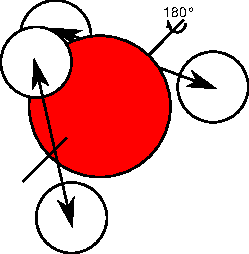
\includegraphics[width=0.25\linewidth]{c2-axis}
    \label{fig:c2-axis}
    }
  \subfigure[$S_4$ axis][$S_4$ axis: $4$-fold rotation-reflection.]{
    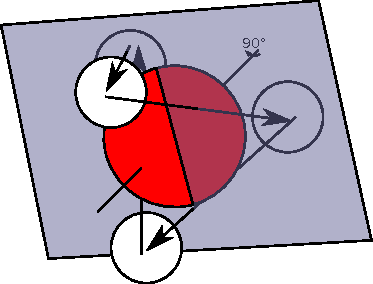
\includegraphics[width=0.4\linewidth]{s4-axis}
    \label{fig:s4-axis}
    }
\newline
  \subfigure[$C_3$ axis][$C_3$ axis: $3$-fold rotation.]{
    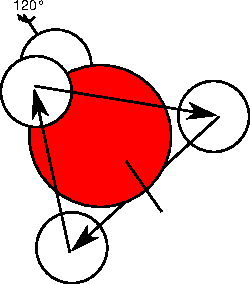
\includegraphics[width=0.25\linewidth]{c3-axis}
    \label{fig:c3-axis}
    }
  \subfigure[$\sigma_\text{d}$ plane][$\sigma_\text{d}$ plane: Mirror plane.]{
    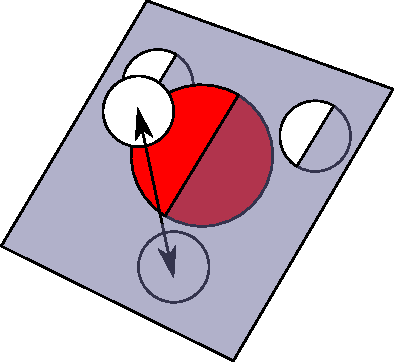
\includegraphics[width=0.4\linewidth]{sigma-plane}
    \label{fig:sigma-plane}
    }
    \parbox{0.85\linewidth}{
      \caption{The possible symmetry operations for a tetraheder, such as the \ce{BH4} unit.
      }
      \label{fig:symmetry}
    }
  \end{center}
\end{figure}

A common notation for symmetry operations is the one attributed to Sch\"onflies~\cite{schonflies-notation-1889} and this notation will be used for discussion of symmetry in this thesis.
~\footnote{See \url{http://en.wikipedia.org/wiki/Schoenflies_notation} for a handy overview of all the Sch\"onflies symbols, including those not mentioned here.}
The relevant symmetry operations are as follow:
\bit
\item $1 \times E$ : Pseudo axis which leaves the system unchanged.
\item $3 \times C_2$ : Axes of 2-fold rotation, enter between each pair of vertices and exit through the opposing pair.
Opposing axes give identical permutations, thus only 3 axes are considered instead of 6.
(\fref{fig:c2-axis})
\item $8 \times C_3$ : Axes of 3-fold rotation, enter through each vertex and exit through the opposing plane, to which the axes are normal. Each axis has 2 operations, forward and backward rotation, which are identical versions of each other.
Thus only 4 unique $C_3$ axes remain.
(\fref{fig:c3-axis})
\item $6 \times \sigma_\text{d}$ : Mirror planes which lie through each pair of vertices with the opposing pair defining the normals.
(\fref{fig:sigma-plane})
\item $6 \times S_4$ : Axes of 4-fold rotation and mirroring which lie identical to the $C_2$ axes with a mirrorplane normal to themselves. Due to the 4-fold rotation, instead of 2-fold, opposing axes give unique permutations.
(\fref{fig:s4-axis})
\eit

When considering only the \ce{BH4} and no environmental effects, the $C$-type operations yield no barrier as the interatomic distances do not vary during the operation.
On the other hand, when performing the mirror-type operations ($\sigma_\text{d}$ and $S_4$), the interatomic distances change, forming a flat \ce{BH4} intermediate, which is very energetically unfavorable.
Due to this difference in intrinsic barriers and the fact that the mirror-type operations aren't, in fact, rotations, only the $C$-type operations have to be considered.

%\begin{figure}
%  \begin{center}
%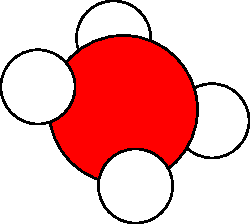
\includegraphics[width=0.2\linewidth]{bh4-flat} % Not included currently but still in git
%  \end{center}
%\end{figure}

